\documentclass[conference, compsoc]{IEEEtran}

\usepackage{graphicx}
\usepackage[UKenglish]{isodate} % for dmy date
\usepackage{blindtext}
\usepackage{fancyvrb} % for code

\RequirePackage[singlelinecheck=off]{caption}
\captionsetup{justification=centering}

\title{\huge{LoRa PHY Range Tests and Software Decoding}}
\cleanlookdateon
\author{Keely Hill\\\today}

% fixes bib use
\def\endthebibliography{%
  \def\@noitemerr{\@latex@warning{Empty `thebibliography' environment}}%
  \endlist}

\begin{document}

\maketitle

\begin{abstract}
LoRa is a recently created patented physical layer protocol for small, low power devices. Networks are being deployed world wide as LoRa WAN (link layer). The attack surface is growing. This project begins by performing range tests of a consumer module physical (PHY) layer. Depending on the settings, up to 5 Km was achieved to transmit a frame -- at the expense of speed. 1 Km was achieved at a more reasonable rate. Along the way, how LoRa functions is discussed. Next and inexpensive RTL-SDR (software defined radio) was used to record raw transmissions from the official PHY module. These transmissions were then attempted (and successfully) demodulated and decoded using GNU Radio and the experimental gr-lora out-of-tree module from Bastille Reasearch. Some common radio vulnerabilities are discussed in relationship with LoRa as a conclusion.
\end{abstract}

\renewcommand\IEEEkeywordsname{Keywords}
\begin{IEEEkeywords}
LoRa, range testing, Software Defined Radio (SDR), physical layer security
\end{IEEEkeywords}

%%%%%%%%%%%%%%%%%%%%%%%%%%%%%%%%%%%%%%%%%%%%%%%%%%%

\section{Introduction}
This is an experimentation project performed with the LoRa physical layer (PHY) using an official consumer LoRa device and software defined radio (SDR). Range testing and successful SDR decoding attempts are performed. As LoRa device networks are deployed around the world, the attack surface grows. It is important to understand what these low powered devices are capable of, and how they function.

\section{LoRa Overview}
LoRa is a patented physical layer chirp spread spectrum modulation format. LoRa operates in license-free bands (433 MHz in Europe, 915 MHz in the US). LoRA WAN is a MAC layer protocol from the LoRa Alliance created as a means to standardize wide area network communications between end-devices\cite{lora-all} using LoRa PHY. It also has the capability to be a gateway to the internet. This paper will focus on LoRa PHY, the physical layer protocol. 

Chirp spread spectrum (CSS) uses the full available bandwidth (e.g. 31.25, 125, 500 KHz) to produce `chirps' of increasing or decreasing frequency. The timing of these chirps are what encode information. They are a major reason why LoRa can operate at long ranges. The `spreading factor' is the number of bits encoded per-symbol (e.g. 7). `Chirp rate' is the slope of the chirp ($df/dt = bandwidth/2^{spreading factor}$). It represents how quickly the frequency is modulated. A larger spreading factor and smaller hamming code rate slows transmission speed while it increases range as it is easier for a receiver to resolve a low power signal. For example, in figure \ref{fig:waterfall-compare}, a steeper slope would equate to a larger spreading factor.

\subsection{Packet format}
The most notable elements of the raw packet is the preamble: initial 8 (or N) up-chirp symbols followed by two down-chirps (for synchronizing). The data then begins. Details on the encoding and modulation are in section \ref{sec:EncAndMod}.

\begin{figure}[htbp]
\begin{center}
\includegraphics[width=1\linewidth]{../img/LoRaTest-Line-of-Site-Map.png}
\caption{Approximate line of site examples (blue) during range tests. Red dot (upper-left) is the transmitter origin.}
\label{line-of-site}
\end{center}
\end{figure}

\section{Range Testing}
Two LoRa transceiver modules where used for range testing\footnote{Adafruit Feather M0 with 900MHz RFM95 LoRa Radio}. The hardware of the radio module is restricted (fundamentally) in frequency -- 868Mhz to 915Mhz for the US band model. The frequency can be adjusted in software, but only that band will work properly.

The `sender' acting as a beacon was programmed to transmit a sequence number, time (seconds) since starting, then delay 10 ms before transmitting again. The total packet size was set to 36. The other `listener' module was programmed to receive the transmission, append the RSSI\footnote{received signal strength indicator}, signal-to-noise ratio, and time in milliseconds since the last packet was received and output the results to the serial port. Each parameter is separated by a comma, thus creating a CSV row that was written to a file.

The RadioHead\cite{radiohead} library was used to interface with the radio modules from Arduino/C++. The radio module used, allowed the setting of `TxPower', which was set to the maximum 23 dBm for these trials.

\

\begin{Verbatim}[fontsize=\small]
/* Sender loop */
void loop() {
    // ...
    sprintf(pckt, "%d,%d,%d,abc123xyz", 
            pcktNum++, miliV(), timeSec());
    
    rf95.send((uint8_t *)radiopacket, 36);
    rf95.waitPacketSent();
    
    //...
    delay(10);
}
\end{Verbatim}

\subsection{Testing Procedure}
Each radio module is connected to a 900Mhz half-wave whip monopole antenna. First, the listener is plugged into a computer running a serial monitor that outputs to a file. This powers the device and starts an infinite loop of listening. The sender is then started by connecting a battery. At the moment the sender is turned on, a GPS recorder app is started on a phone. Later, the two datasets are combined to calculate the distance from origin.

\subsection{Testing Location}
These experiments took place over a period of a few weeks in central Florida with transmissions occasionally going through vegetation. Humidity was at least above 50\% and not controlled for. The transmitter was placed next to a fifth-story window facing the direction of reception. Direct line of site (no major structural occlusions) was more-or-less constant.

Table \ref{tab:tested-settings} lists the radio settings included in RadioHead that were tested. Due to the nature of the PHY layer protocol, the larger the spreading factor (thus longer range), the slower the transmission.

\subsection{Testing Results}
Figure \ref{results-chart} shows a summary of the results obtained from the range testing. One-way range is what mattered in these tests, so packet acknowledgments were not used to determine failed transmissions. Instead, `missed packets' were determined by the sequence number included in each packet during data processing.

It is clear that the longest setting tested (12 spreading factor) can easily be received 5 Km away with minimal packet loss -- at the detriment of speed. It took about 2.7 seconds to transmit the 36 byte packet; about 104 bps. Compare this to the medium range (7 spreading factor) that would start dropping packets at 500 meters (and loose all at 900 meters) with a transmit time of 86 milliseconds; 3428 bps. It is important to consider that this is a physical layer test, so payload data rate will decrease as headers are added down the stack or number of parity bits increased.

~1 Km and 5 Km is impressive for such a small low power module and antenna running on a  battery. Current draw is about 300uA during full sleep, and about 120mA peak during transmit according to the manufacturer\cite{ada-lora}. Using amplifiers and/or a directional antenna would only increase this range. 

%% Water fall compare figure
\begin{figure}[htbp]
\begin{center}
\includegraphics[height=8.5cm]{../img/Range-Power-compare.png}
\caption{\textit{Left}: A waterfall spectrogram a far distance from the transmitter. \textit{Right}: waterfall of the start of a LoRa PHY packet with preamble and 2 sync-chirps about a meter from the transmitter.}
\label{fig:waterfall-compare}
\end{center}
\end{figure}

%% Bandwidth RadioHead Table
\begin{table*}[htp]
\normalsize
\caption{Tested LoRa Settings}
\begin{center}
\begin{tabular}{ c c c c c }
Bandwidth & Hamming & Spreading & Claimed & Measured \\
(kHz) &  & {\small(symbols/chirp)} & Range & bps ($\pm 1$) \\
\hline
125 & 4/5 & 7 & medium & 3,428 \\
31.35 & 4/8 & 9 & long & 175 \\
125 & 4/8 & 12 & longer & 104 \\
\end{tabular}
\end{center}
\label{tab:tested-settings}
\end{table*}%

%% Results Chart
\begin{figure*}[]
\begin{center}
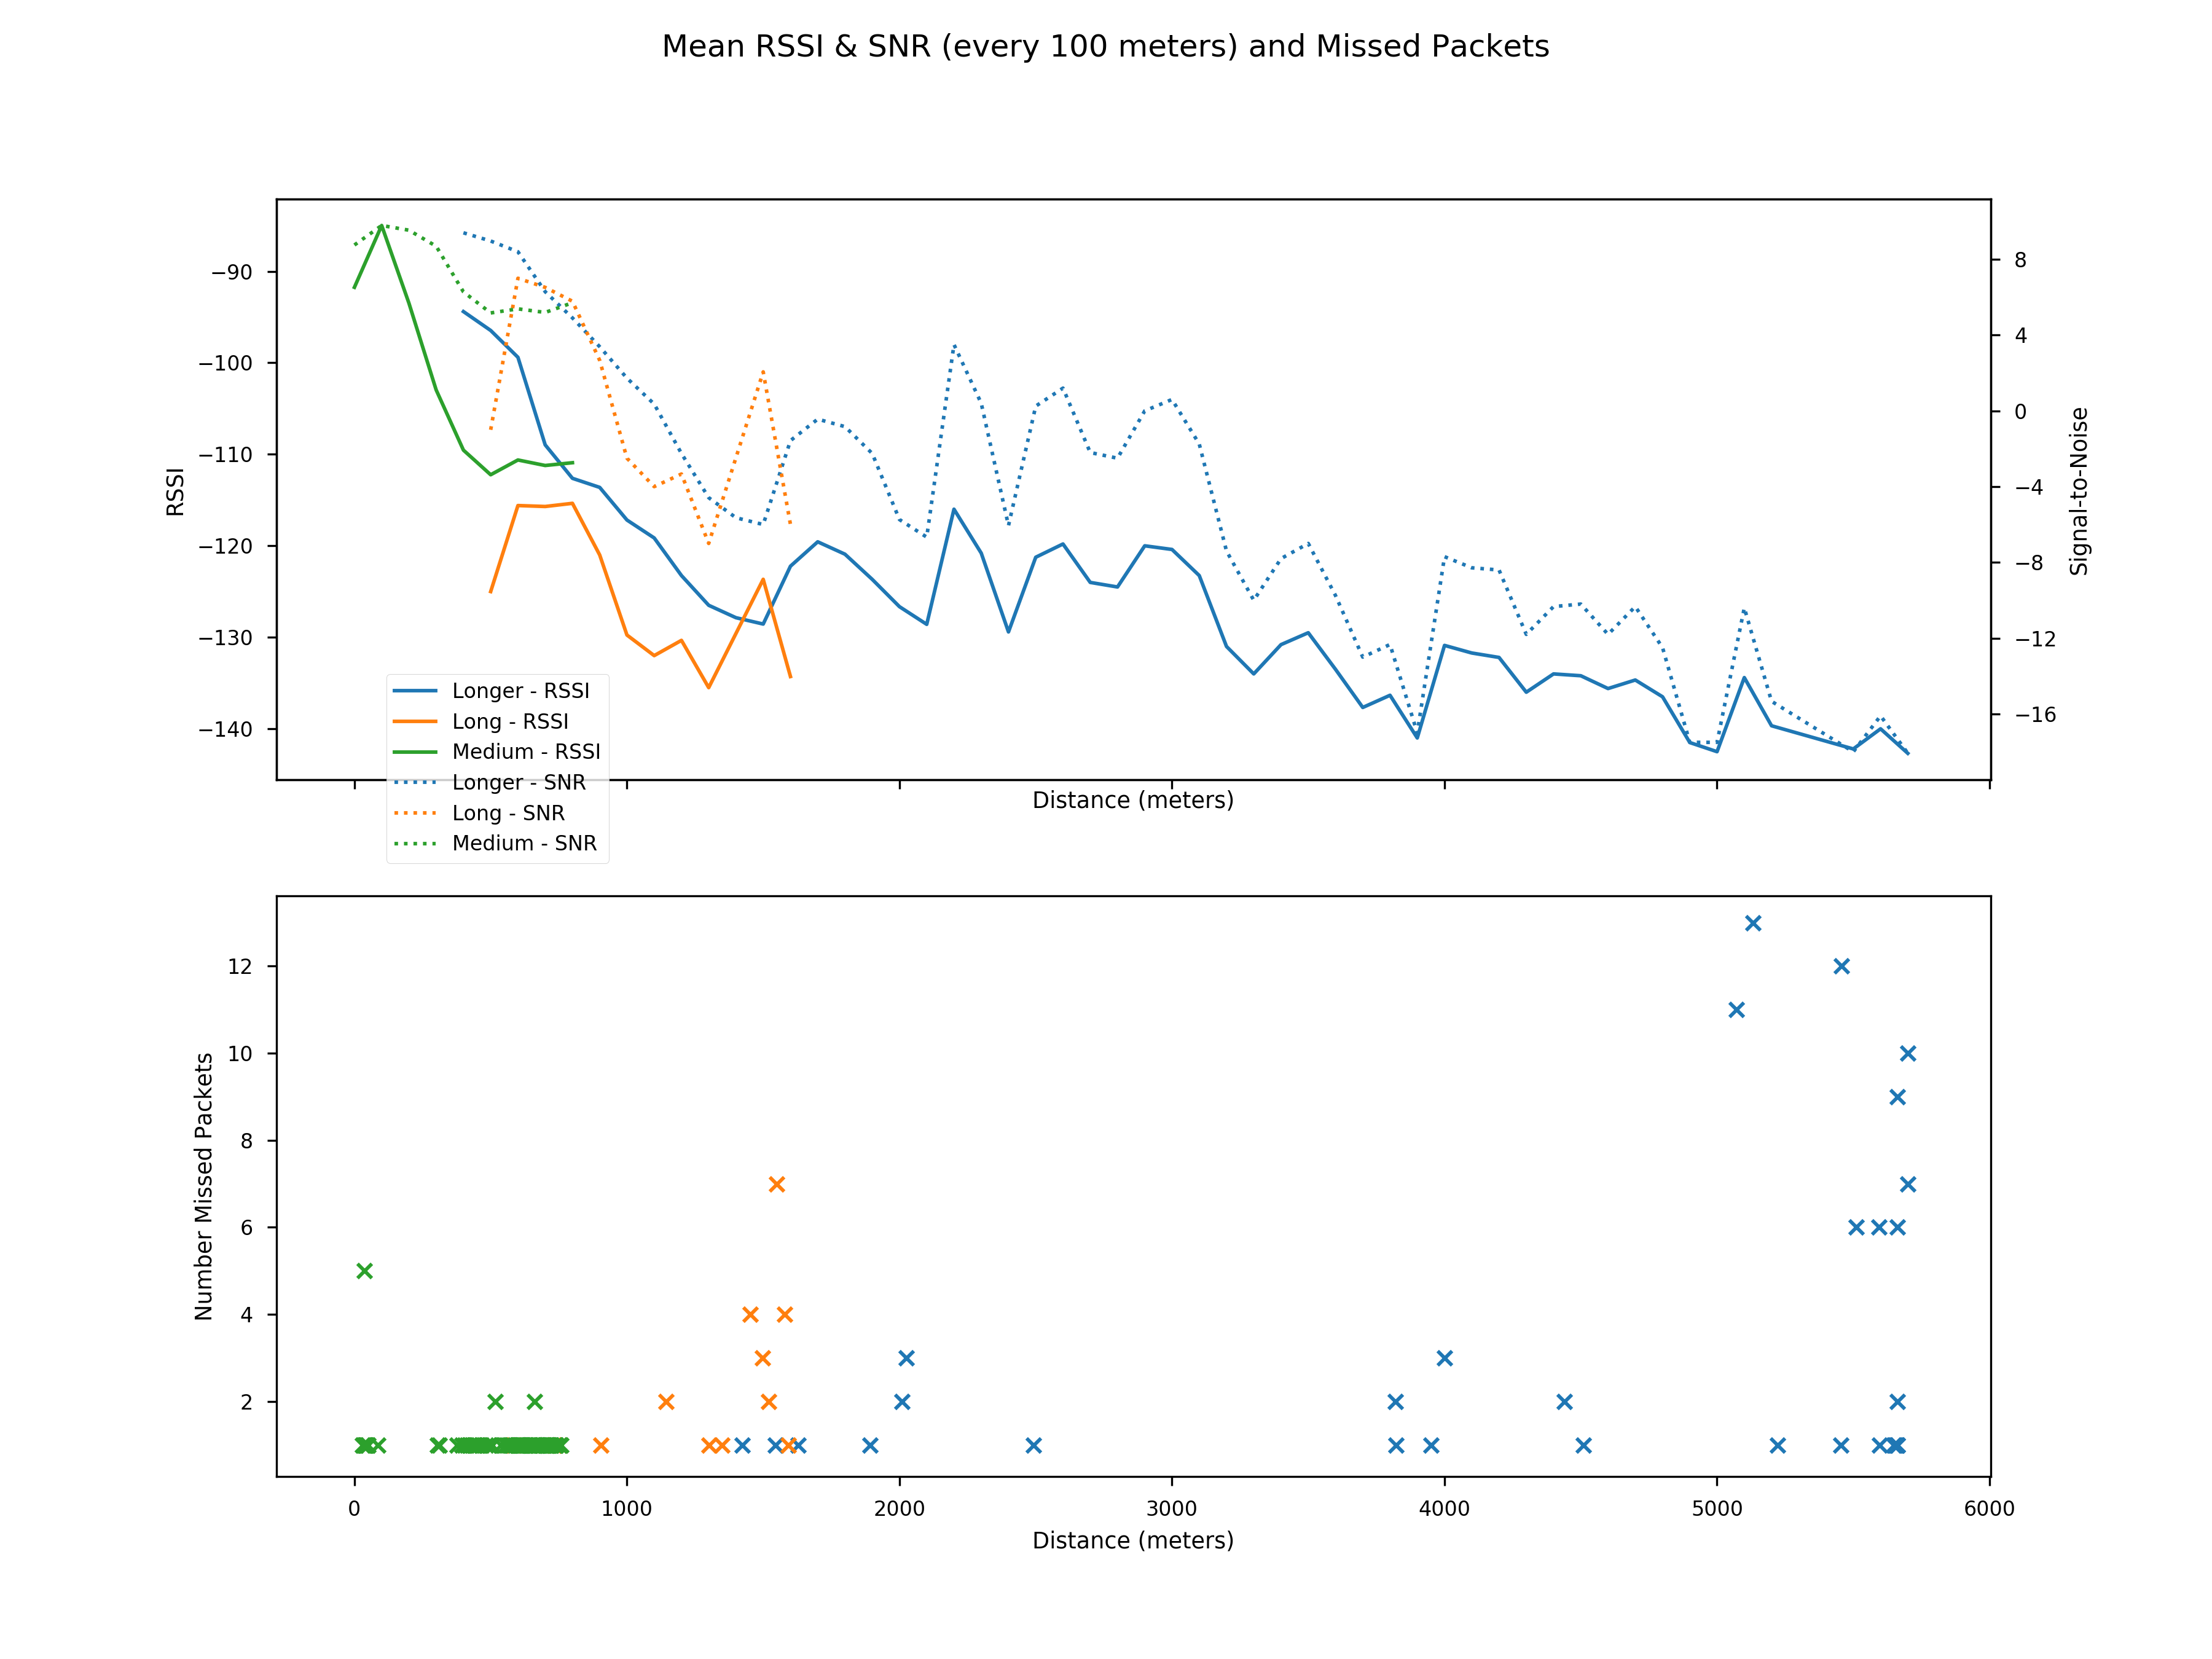
\includegraphics[width=\linewidth]{../img/processed_RSSI_SNR_Missed.png}
\caption{(upper) Mean RSSI \& SNR every 100 meters and (lower) Missed Packets}
\label{results-chart}
\end{center}
\end{figure*}

\section{Waterfall Visualization}
Most SDR software has a waterfall visualization component. It is a graph overtime (axis 1) of the frequency's (axis 2) amplitude (axis 3, usually color intensity). High spreading factor chirps can very easily be seen when it is updating fast enough. Figure \ref{fig:waterfall-compare} shows a similar transmission received from far away and near by. The ability to view the waterfall of a signal gave the ability to check that the a signal was actually being received at the desired frequency and bandwidth when first starting analysis. Due to limitations in the SDR used and computer processors speed, only the transmissions with spreading factor of 12 could resolve individual chirps live using the CubicSDR software. Other smaller spreading factor settings were nonetheless obvious from the water fall as their power dominated the band. The other spreading factors were still able to be resolved to chirps by throttling a raw ``IQ" file after recording it with a small GNU Radio flow graph (discussed later in section \ref{sec:gr-record}, figure \ref{fig:rtl-gr-recorder}).

\section{LoRa PHY Encoding and Modulation}
\label{sec:EncAndMod}

Much of the summarized information in this section was discovered experientially or otherwise by M. Knight and the Bastille Threat Research Team (Bastille)\cite{grcon}. An understanding of how official LoRa radios encode and modulate data is essential to decoding the raw signal and realizing its long range ability.

\subsection{De-chirping}
A symbol is represented as a instant change in frequency of a chirp back to the lower frequency. By multiplying a symbolic chirp by a locally generated opposite chirp and taking a $2^{spreading factor}$ bin Fast Fourier Transform(FFT), the bin index with the greatest amplitude contains the encoded symbol. This is \textit{not a bit or byte}, next it must be decoded.

\subsection{Preamble and Start of Frame}
The preamble (a number of continuous up-chirps) and start of frame delimiter (two down-chirps) indicate the start of a data frame. After being de-chirped, consecutive FFT bins with the same symbol indicate the preamble. The two synchronization down-chirps are de-chirped similarly using overlapping FFTs to improve temporal resolution for synchronization (since it is more computationally expensive).

\subsection{Whitening and Interleaving}
Data whitening purposely introduces randomness into the symbols for other features (like clock recovery) that would be implemented by a receiver. True symbols are extracted with an XOR operation. \texttt{gr-lora} experimentally determined the whitening sequence by transmitting zeros.

Interleaving scrambles bits to make received data stronger against bursts of interference. Knight claims that the interleaver described in a patent filing is not implemented by the standard and concluded that it uses a type of diagonal interleaver\cite{grcon}.

\subsection{Forward Error Correction}
LoRa uses Hamming codes as a means to correct bits flipped in transit by adding redundancy to the transmission. LoRa uses a fractional representation: 

\begin{equation}
\frac{\# data bits}{\# data bits + \# parity bits}
\end{equation}
\ %br

For example: 4/5; a total of 5 bits encodes 4 data bits. See the `Hamming' column in Table \ref{tab:tested-settings} for some used by the RadioHead library for LoRa capable radios. LoRa has the bits in nonstandard order that must be adjusted before fully decoding. The result of applying forward error correction is the actual data of the PHY packet.

\section{Software Defined Radio}
A software defined radio (SDR) abstracts radio circuity to be implemented by software instead. The hardware component is an analog to digital converter. This makes SDRs incredibly flexible -- especially when dealing with scanning local frequencies and doing custom signal processing on them. For this project, an inexpensive RTL-SDR\footnote{SDR Model: R820T2 RTL2832U 1PPM TCXO SMA V3 Dongle} dongle was used.

\section{Decoding with SDR}

\subsection{GNU Radio}
GNU Radio\cite{gnuradio} is a free(libre) software tool for interfacing with SDRs and performing signal processing on the input. It comes with many ``blocks" of processing that are connected together to form a ``flowgraph". Example blocks include: FM (De)modulation, low pass filter, FFT, WAV file sink, and GUI waterfall sink. These flowgraphs are `compiled' to a Python script to be run. Custom blocks can be written in Python or C++ (as a class) an integrated into a flowgraph. In this project GNU Radio is used to perform the actual decoding of LoRa packets in a frequency flexible way. GNU Radio was installed on a Debian machine for this project.

As mentioned previously, SDR allows the recoding of raw ``IQ" signals for later processing. This is a technique used for feeding signals into GNU Radio that are attempting to be decoded. It makes it simple to pre-record various transmissions with the ability to later switch between and throttle them (making it easier on the processor).

\subsection{Recording IQ Files}
\label{sec:gr-record}
To make decoding attempts easier to perform, raw IQ (In-phase/quadrature) signals were recorded using a simple GNU Radio flowgraph (figure \ref{fig:rtl-gr-recorder}). IQ signals are a means of digitally storing samples of radio data as two amplitude modulated sinusoids without the loss of information. These files are later used as a source for demodulating and decoding flowgraph (figure \ref{fig:gr-decode-graph}).

% GR Recorder graph
\begin{figure}[htbp]
\begin{center}
\includegraphics[width=7cm]{../img/RTL-gr-recorder-graph.png}
\caption{The left RTL `source' block pipes the data into an output file (sink) and a live GUI waterfall.}
\label{fig:rtl-gr-recorder}
\end{center}
\end{figure}

\subsection{\texttt{gr-lora} out of tree (OOT) module}
\texttt{gr-lora} is an OOT module for GNU Radio. It is a (limited) open source implementation of LoRa based on blind signal analysis by Matt Knight and Bastille. It is used as a stepping off point for this paper.


\begin{figure*}[]
\begin{center}
\includegraphics[width=15cm]{../img/success1-GR-decode-graph.png}
\caption{Flowgraph used to decode LoRa signals. The `variable' blocks are used to match signal parameters.}
\label{fig:gr-decode-graph}
\end{center}
\end{figure*}

\subsection{Switching Transmitter Library}
After multiple failed attempts to demodulate a signal using gr-lora (before even decoding), reading past issues on GitHub lead to the discovery that gr-lora only supports ``implicit header" mode -- the whitening sequences are different. Since RadioHead only supports ``explicit header" mode, the Arduino based transmitter software was switched\footnote{RadioHead was originally used due to its general popularity, greater chip support, the fact that sending a packet does not block code execution, and unawareness of the arduino-LoRa library at the time.} to use Sandeep Mistry's ``Arduino LoRa" library\cite{sandeep}. It allows more control of the LoRa header, spreading factor, bandwidth, and hamming code rate. Using this library, something like the following can be setup (full code in appendix):

\begin{Verbatim}

LoRa.setSpreadingFactor(7);
LoRa.setSignalBandwidth(125E3);
LoRa.setCodingRate4(5); // 4/5

// ...

LoRa.beginPacket(true); // implicit header
uint8_t pkt[] = {0x12,0x34,0x56,0x78,0x9a};
LoRa.write(pkt, 5);
LoRa.endPacket(); // block & transmit
\end{Verbatim}


\subsection{Decoding Flowgraph}
Figure \ref{fig:gr-decode-graph} displays the GNU Radio flowgraph used to successfully demodulate and decode LoRa PHY signals. The design is based on examples provided by gr-lora. Two blocks handle the \textit{demodulating} and \textit{decoding} individually (chirps to symbols and symbols to bytes, respectively). It did not always decode perfectly, at times a few bits were incorrect. From online discussion, the issue seems to come from the de-interleaver not being ideal. The major of decoding is correct.

\section{Importance of physical layer security}

The physical layer is the fundamental component of all communication systems. The wireless physical layer is exposed to the world by its very nature -- it is ubiquitous and vulnerable. No matter encryption, a simple spectrogram will show if and when a communication is occurring in some radius around the evesdropper. As the number of wireless devices and sensors increases, so does the attack surface. Therefore securing this layer is important to securing the rest of the stack for commercial, military, scientific, emergency, and human rights usage. 

\subsection{Packet in Packet}

The proclaimed ``Packet in Packet" attack\cite{pkt-in-pkt} is a method for indiscriminately embedding physical layer data frames via upper layer protocols by abusing standard compliant preambles and error correction. This method can avoid intrusion detection systems and firewalls. 

Essentially, the entire physical layer packet data is embedded into, say, a link layer frame. When a crafted error occurs on the link layer frame's checksum, the physical layer (and possibly malicious) packet is interpreted instead. The start of frame delimiter in IEEE 802.15.4 (e.g. Zigbee) is simply a specific byte (\texttt{xA7}), so it can be placed in upper layer payloads.

LoRa uses two reverse chirps, a `symbol' that can't exist in upper layers, it is only used to sync a receiver with an incoming signal's data. This is strong resistance against this particular attack. 

\subsection{Device Dialects (vulnerability)}
There are slight (but still standard compliant) implementation differences in some commercial IEEE 802.15.4 radio chips. These `dialects' --as the researchers coined-- allow the transmission of packets that can only be `heard' by specific devices, thus never being received by any other radios. That includes intrusion detection devices on a wireless network.\cite{dialect}

\subsection{Jamming}
Radio jamming is one of the simplest and effective techniques of preventing availability. It is the physical layer equivalent of denial of service. LoRa is susceptible to selective jamming where ``a malicious jammer can systematically jam either a particular type of message or all messages coming from a particular end-device." \cite{lora-jam}

There are two methods that change the spreading factor to resist this attack: (1) Use a large spreading factor --like 12-- to "beat" the jammer RSSI and (2) reduce an attacker's reaction time by using a small spreading factor, thus being ``in the air" for a shorter duration.

\section{Further Work}
As it developed, this research and paper became a combination survey-experimentation of LoRa knowledge. Scanning a range of frequencies for a LoRa signal (and attempting to determine its parameters like spreading factor and bandwidth) may be an interesting next step, but a more difficult undertaking. The implementation of more PHY features (such as explicit header whitening and clock recovery) in OOT modules, like gr-lora, should also be continued. Further improving the physical layer and implementing the LoRa WAN (link layer) would be interesting future investigations. 

Continuing to investigate packet in packet, potential device dialects, and any other security vulnerabilities would obviously also be important work.

\section{Concepts Learned}
I have been wanting to experiement with SDRs for some time. This project gave me the nudge to get started. Thusly, I learned the basics of SDRs, how they work, and how they interact with radio waves. The ability to visualize and `play' with signals also gave me a much greater intuition of the radio spectrum.

This ability came from the GUI listening software (e.g. CubicSDR, GQRX) and GNU Radio. I also learned the basics of GNU Radio, its patterns, the functions of different blocks, and how wiggling one thing affects another.

I also learned a lot about physical layer protocols in general -- partly from a visual intuition perspective with spectrograms and partly from a mathematical one with IQ and (de)modulation. Of course, I also learned (in more detail) how LoRa PHY works, and what it is capable of.

\section{Conclusion}
This project demonstrated the range and data speed of inexpensive low power LoRa radios. It also (after several failed attempts) worked to understand and decode signals from an official transceiver using an inexpensive SDR dongle and GNU Radio. The physical layer attack surface is ever growing -- it is important to understand and secure it.

\newpage % shift to next column to even out

\section{Acknowledgments}
The idea of this project came from my participation in FL Polytechnics's ASTRO Rocket Design club. I have been working on a long distance (at least 3000 meters) payload telemetry system. I started programming for these LoRa modules purchased by the club in the previous semester. We are using the same two-radio reception system described in section 3 (Range Testing). I thought it would be nice to also have a more extensible model for potential future use (multiple receivers with different antennas for redundancy). I combined these goals into this project.

Additionally, Matt Knight's research and conference talks were a great starting point for this project.

%%%%%%%%%%%%%%%%%%%%%%%%%%%%%%%%%%%%%%%%%%%

\bibliographystyle{IEEEtran} % unsrt
\bibliography{refs}

\clearpage
\section*{Appendix}

\subsection*{\texttt{arduino-LoRa} Transmitter Code}
\begin{Verbatim}[fontsize=\footnotesize]
/* main.cpp */

#include <SPI.h>
#include <LoRa.h>

#define RFM95_CS 8
#define RFM95_RST 4
#define RFM95_INT 3

#define RF95_FREQ 915E6

#define LED_WHEN_TRANSMITTING LED_BUILTIN

unsigned long startTransTime;

void setup() {
	pinMode(RFM95_RST, OUTPUT);
	digitalWrite(RFM95_RST, HIGH);

	Serial.begin(9600);

	// manual reset
	digitalWrite(RFM95_RST, LOW);
	delay(10);
	digitalWrite(RFM95_RST, HIGH);
	delay(10);

	// SPI pins setup
	LoRa.setPins(RFM95_CS, RFM95_RST, RFM95_INT);

	if (!LoRa.begin(RF95_FREQ)) {
    	Serial.println("Starting LoRa failed!"); while (1);
  	}
	Serial.println("OK LoRa radio init.");

	LoRa.setSpreadingFactor(8);
	LoRa.setSignalBandwidth(125E3);
	LoRa.setCodingRate4(5); // 5-8, inclusive
	LoRa.setPreambleLength(8);
}

void loop() {
	Serial.print("Sending...");
	digitalWrite(LED_WHEN_TRANSMITTING, HIGH);
	startTransTime = millis();

	LoRa.beginPacket(true); // true for implicit header
	uint8_t pkt[] = {0x12,0x34,0x56,0x78,0x9a,0x00};
	LoRa.write(pkt, 6);

	bool hadSuccess = LoRa.endPacket();

	Serial.print("Success?: ");
	Serial.println(hadSuccess);

	digitalWrite(LED_WHEN_TRANSMITTING, LOW);
	Serial.print("Done transmitting, ");
	Serial.print((float)(millis() - startTransTime) / 1000);
	Serial.println(" sec. to complete.\n");

	delay(500);
}
\end{Verbatim} % appendix.tex

\end{document}


